\chapter{Previous Designs and Implementations}\label{sec:previous-designs}

% Describe implementations in the past tense.

Before working on ShareTrace, I did not have experience developing distributed algorithms. The approach proposed in \Cref{ch:risk-propagation} is my \emph{fifth} attempt at defining a performant implementation of risk propagation that is also decentralized and online. The prior four attempts offered valuable learnings that guided me toward the proposed approach; however, only the latter supports truly decentralized, privacy-preserving contact tracing. To document my efforts in developing this thesis, prior designs and implementations are provided in this appendix.

\section{Thinking Like a Vertex}\label{sec:giraph}

The first iteration of risk propagation\footnote{\url{https://github.com/cwru-xlab/sharetrace-giraph}} utilized Apache Giraph\footnote{\url{https://giraph.apache.org}}, an open-source version of the iterative graph-processing library, Pregel \citep{Malewicz2010}, which is based on the bulk synchronous parallel model of distributed computing \citep{Valiant1990}. Giraph follows the \define{``think like a vertex'' paradigm} in which the algorithm is specified in terms of the local information available to a graph \vertexName{} \citep{McCune2015}.

Risk propagation was implemented as defined by \citet{Ayday2020,Ayday2021}, using the factor graph representation of the contact network. Moreover, the implementation assumed the use of Dataswyft Personal Data Accounts\footnote{\url{https://www.dataswyft.io}}, which provide a data-oriented interface to self-sovereign identity \citep[pp. 98--99]{Preukschat2021}. However, because the Exposure Notification API developed by Apple\footnote{\url{https://covid19.apple.com/contacttracing}} and Google\footnote{\url{https://www.google.com/covid19/exposurenotifications}} does not permit remotely persisting ephemeral identifiers, the implementation assumed that user geolocation data would be analyzed to generate the factor \verticesName{} in the factor graph (\Cref{sec:location-based}). \Cref{fig:aws-architecture} describes the high-level architecture. Callouts 1, 2, and 4 were implemented using a fan-out design in which a \define{ventilator} Lambda function divides the work amongst \define{worker} Lambda functions.

\begin{figure}[htbp]
\centering
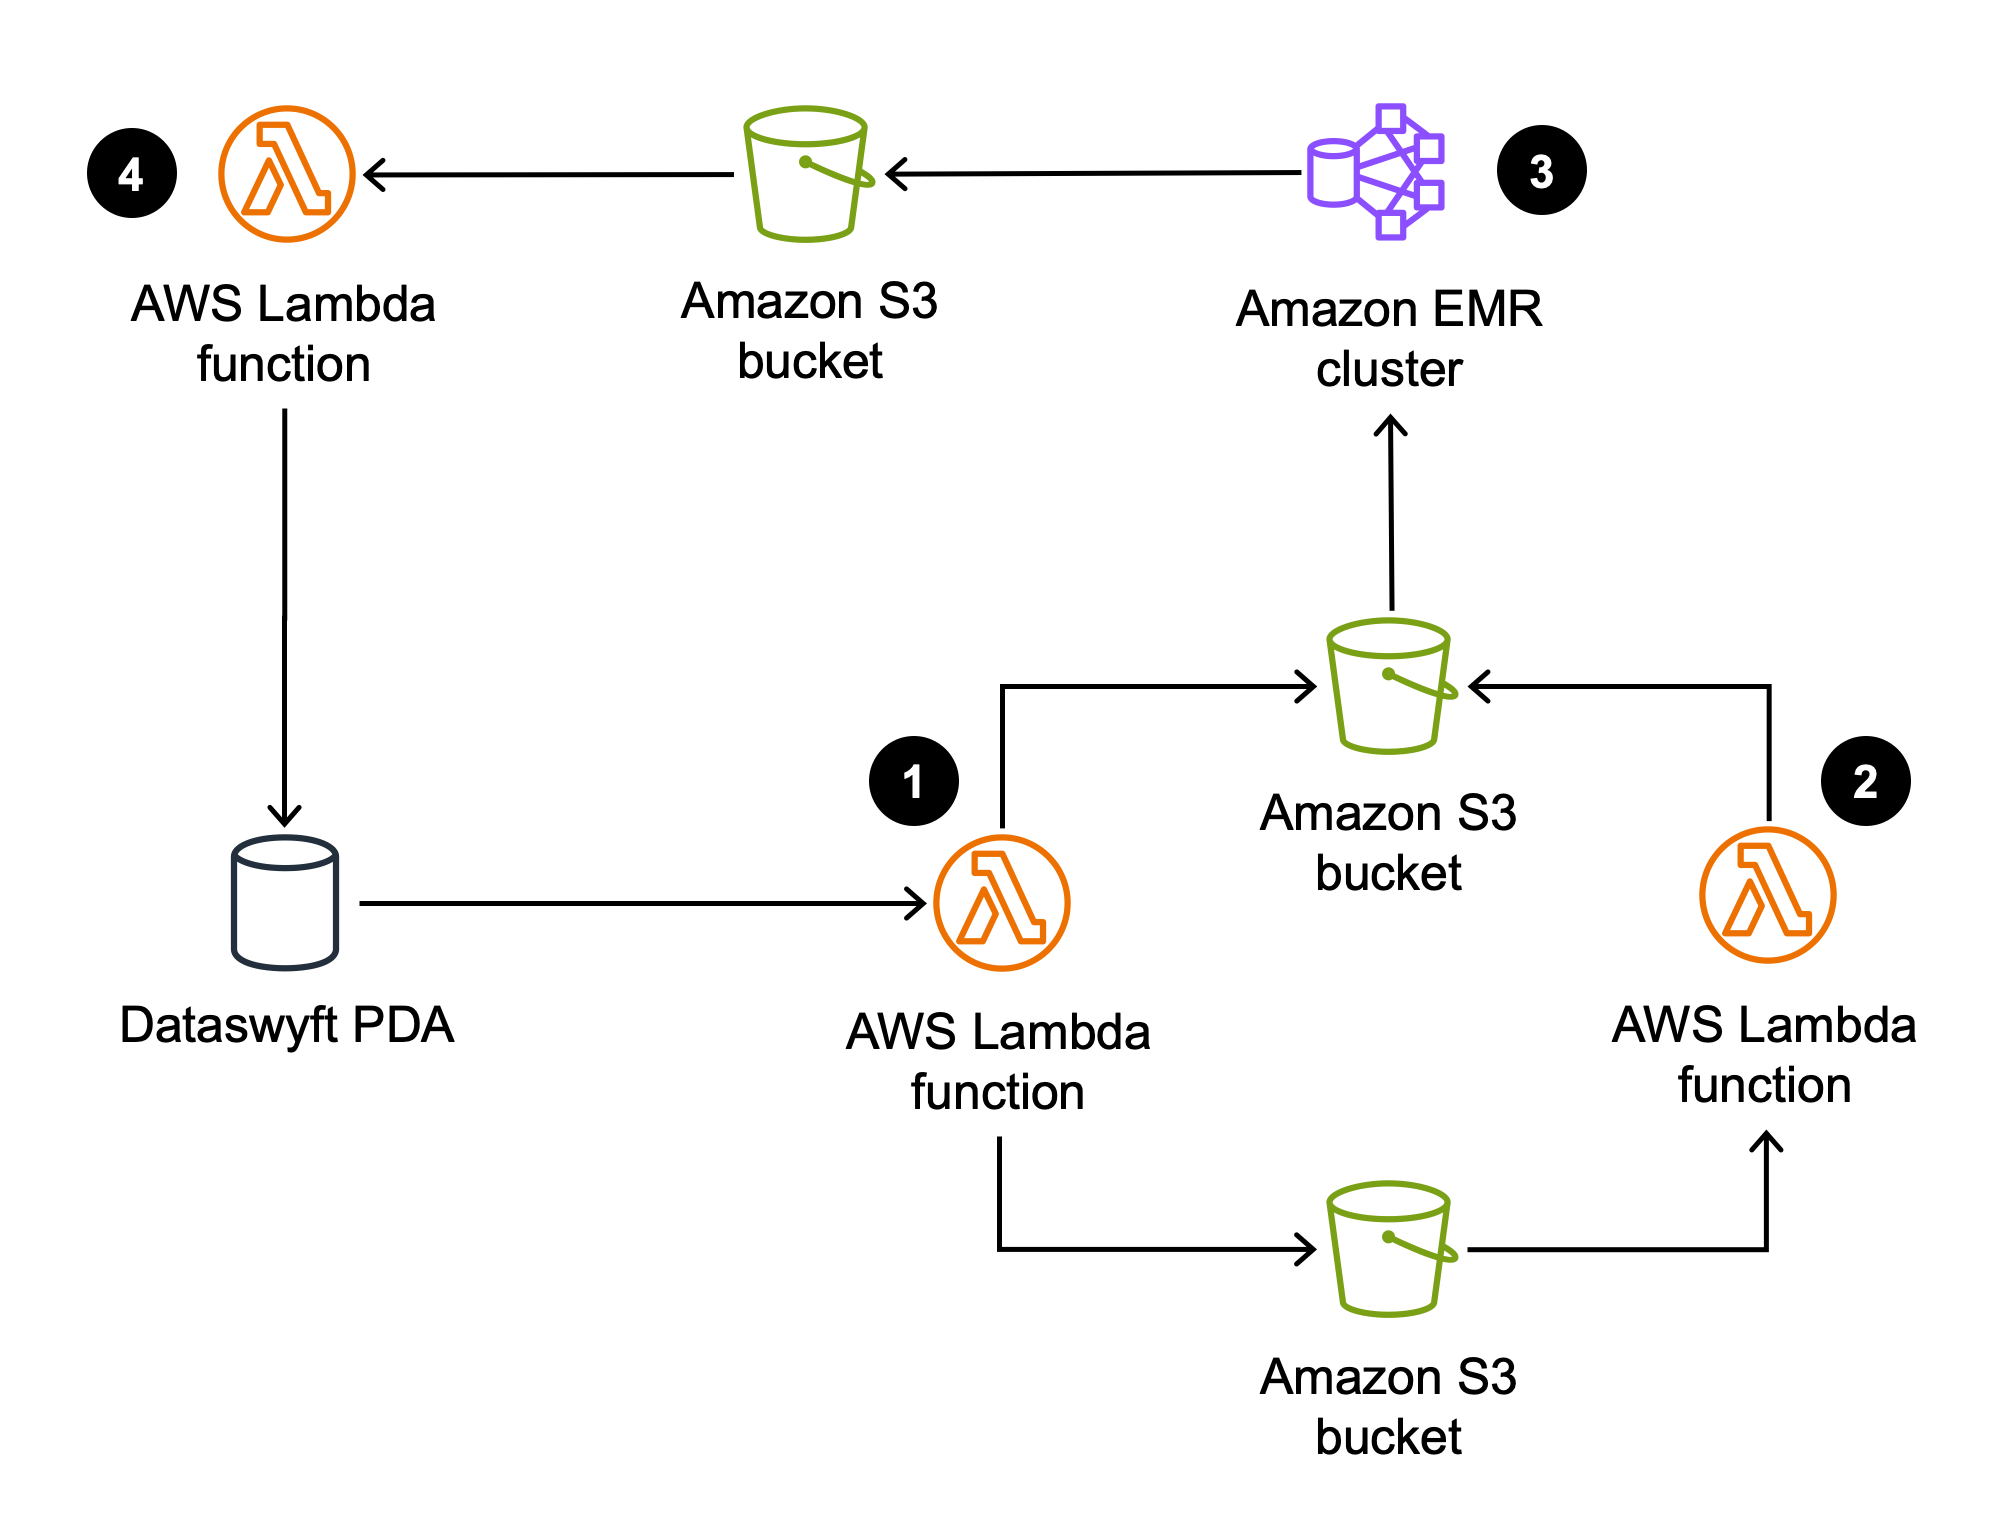
\includegraphics[width=\textwidth]{aws-architecture}
\caption[ShareTrace batch-processing architecture]{ShareTrace batch-processing architecture. \ding{202} An AWS Lambda function\protect\footnotemark{} retrieves the recent risk scores and location data from the Dataswyft Personal Data Accounts (PDAs) of ShareTrace users. Risk scores are formatted as Giraph \verticesName{} and stored in an Amazon Simple Storage Service\protect\footnotemark{} (S3) bucket. Location data is stored in a separate S3 bucket. \ding{203} A Lambda function performs a contact search over the location data and stores the contacts as Giraph edges in the same bucket that stores the Giraph \verticesName. \ding{204} Amazon Elastic MapReduce\protect\footnotemark{} (EMR) runs risk propagation as a Giraph job and stores the exposure scores in an S3 bucket. \ding{205} A Lambda function stores the exposure score of each user in their respective PDA.}
\label{fig:aws-architecture}
\end{figure}

\addtocounter{footnote}{-1}
\addtocounter{footnote}{-1}
\footnotetext[\thefootnote]{\url{https://aws.amazon.com/lambda}}
\addtocounter{footnote}{1}
\footnotetext[\thefootnote]{\url{https://aws.amazon.com/s3}}
\addtocounter{footnote}{1}
\footnotetext[\thefootnote]{\url{https://aws.amazon.com/emr}}

\clearpage

A couple factors prompted me to search for an alternative implementation.
  \begin{enumerate}
    \item \emph{Dependency management incompatibility}. The primary impetus for reimplementation was the dependency conflicts between Giraph and other libraries. Despite several attempts (e.g., using different library versions, using different versions of Giraph, and forcing specific versions of transitive dependencies) to resolve the conflicts, a lack of personal development experience and stalled progress prompted me pursue alternative implementations.
    \item \emph{Implementation complexity}. For a relatively straightforward data flow, the architecture in \Cref{fig:aws-architecture} corresponded to over 4,000 lines of source code. In retrospect, AWS Step Functions\footnote{\url{https://aws.amazon.com/step-functions}} could have been used to orchestrate the workflow, including the fan-out design pattern, which would have simplified the Lambda function implementations. Regarding the implementation of risk propagation, one-mode projection (first used in \Cref{sec:projected-subgraphs}) would have simplified the implementation since it avoids types of \verticesName{} and messages.
  \end{enumerate}

\section{Factor Subgraph Actors}\label{sec:subgraph-actors}

In an attempt to simplify the design in \Cref{sec:giraph}, I rewrote risk propagation using the Ray Python library\footnote{\url{https://www.ray.io}}. While it claims to support actor-based programming, Ray only offers coarse-grained concurrency, with each actor being mapped to a physical core. To achieve parallelism, the factor graph was partitioned amongst the actors such that each actor maintained a subset of variable \verticesName{} \emph{or} factor \verticesName. The graph topology was stored in shared memory since it was immutable. The lifetime of this design was brief for the following reasons.
  \begin{enumerate}
    \item \emph{Poor performance}. Communication between Ray actors requires message serialization. Moreover, partitioning the factor graph into subsets of factor \verticesName{} and variable \verticesName{} results in maximal interprocess communication. Unsurprisingly, this choice of partitioning manifested in poor runtime performance.
    \item \emph{Design complexity}. Not using a framework, like Giraph, meant that this implementation required more low-level code to implement actor functionality and message passing. Regardless of the performance, the overall design of this implementation was poorly organized and overthought.
  \end{enumerate}

\section{Driver-Monitor-Worker Framework}\label{sec:mwd-framework}

Based on the poor runtime performance and complexity of the previous approach, I speculated that centralizing the mutable aspects of risk propagation (i.e., the iterative exposure scores of each variable \vertexName) would improve both metrics. With this is mind, I designed the \define{monitor-worker-driver} (MWD) \define{framework}, which draws inspiration from the \define{tree of actors} design pattern\footnote{\url{https://docs.ray.io/en/latest/ray-core/patterns/tree-of-actors.html}}. \Cref{fig:mwd-framework} describes the framework.

\begin{figure}[htbp]
\centering
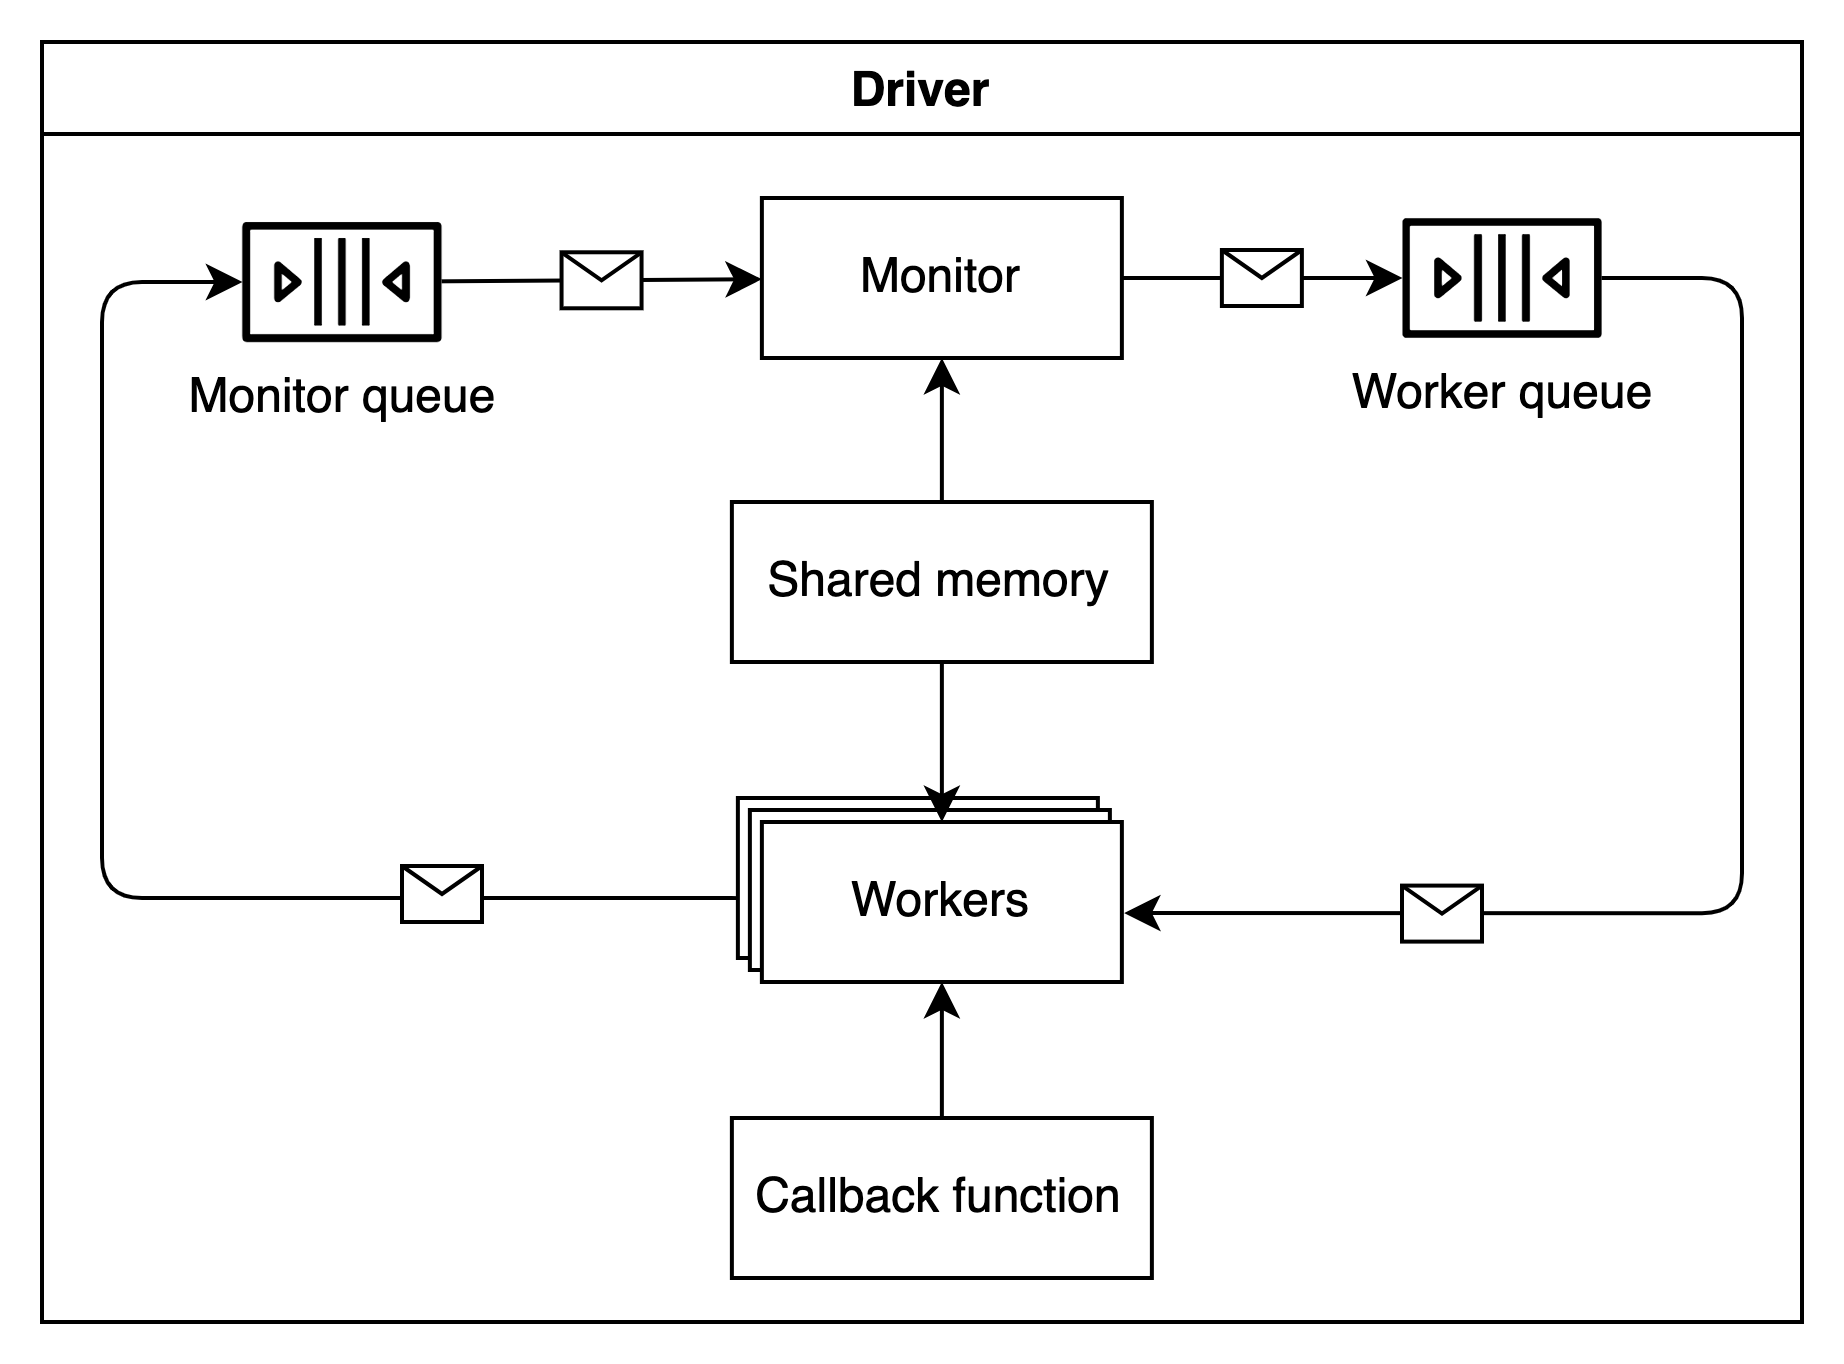
\includegraphics[width=\textwidth]{mwd-framework}
\caption[Monitor-worker-driver framework]{Monitor-worker-driver framework. The \define{monitor} encapsulates the mutable state of the program and decides which messages are processed by workers. A \define{worker} is a stateless entity that processes the messages that the monitor puts in the \define{worker queue}. Worker behavior is defined by a \define{callback function}, which typically depends on the message contents. The side effects of processing a message are recorded as new messages and put in the \define{monitor queue}. This cycle repeats until some termination condition is satisfied. Any immutable state of the program can be stored in \define{shared memory} for efficient access. The \define{driver} is the entry point into the program. It initializes the monitor and workers, and then waits for termination.}
\label{fig:mwd-framework}
\end{figure}

For risk propagation, the driver creates the factor graph from the set of risk scores $\vScores$ and contacts $\vContacts$, stores the factor graph in shared memory, sets the initial state of the monitor to be the maximum risk score of each individual, and puts all risk scores in the monitor queue. During message passing, the monitor maintains the exposure score for each variable \vertexName.

The MWD framework was the first approach that utilized the send coefficient to ensure the convergence and termination of message passing. However, because the MWD-based implementation assumed the factor graph representation of the contact network, the send coefficient was applied to both variable and factor messages.

Compared to \Cref{sec:subgraph-actors}, this implementation provided a cleaner design and less communication overhead. However, what prompted (yet another) an alternative implementation was its scalability. Because the monitor processes messages serially, it is a bottleneck for algorithms in which the workers perform fine-grained tasks. Indeed, the Ray documentation\footnote{\url{https://docs.ray.io/en/latest/ray-core/patterns/too-fine-grained-tasks.html}} notes that the parallelization of small tasks is an anti-pattern because the interprocess communication cost exceeds the benefit of multiprocessing. Unfortunately, the computation performed by factor \verticesName{} and variable \verticesName{} was fine-grained, so the scalability of the MWD framework was demonstrably poor.

\section{Projected Subgraph Actors}\label{sec:projected-subgraphs}

The last alternative design of risk propagation is the subject of published work \citep{Tatton2022b} and preprint \citep{Tatton2022a}. Since those works were written during the coarse of my graduate studies, algorithmic details and experimental results are included below.

\subsection{Risk Propagation}

Like all previous designs, risk propagation is an offline algorithm. Let $\pNumberOfSubgraphs$ be the number of actors, where $\vGraph_i$ represents \indexed{i}{subgraph of contacts} that is associated with \indexed{i}{actor}. It is assumed that actor communication is expensive, so a partitioning algorithm \citep{Buluc2016} that minimizes communication complexity between actors is key to maximizing performance. Each actor is associated with a \define{remote mailbox} and a \define{local mailbox}. The former is designated for messages sent by other actors, while the latter is designated for messages associated with individuals within the same subgraph. For an actor to send a message to another actor, it must know the address of the target actor's remote mailbox and an identifier of the individual within the target actor's subgraph. The \cRiskPropagationMain{} operation describes the main steps.

\begin{function}{\nRiskPropagationMain}[\vScores, \vContacts]
  \State $\vGraph \assign \Call{Contact-Network}{\vContacts}$
  \ForEach{$i \in \intRange{1}{\pNumberOfSubgraphs}$}
    \State $\cRiskPropagationActor[\vGraph_i, \vScores_i]$
  \EndFor
  \State Collect the exposure scores from all actors
\end{function}

The \cRiskPropagationActor{} operation defines the behavior of an actor. According to \citet{Tatton2022a,Tatton2022b}, an actor terminates when no message has been received after a set period of time. \citet{Tatton2022a} also allows an actor to terminate after passing messages for a maximum duration; or if a certain number of messages have been received and none caused an individual's exposure score to be updated. Compared to asynchronous risk propagation (\Cref{sec:asynchronous}), actor behavior differs in two significant ways:
\begin{enumerate}
  \item The send threshold is applied \emph{across} contacts and discriminates against risk scores that are newer than the initial risk score. The latter is based on the assumption that newer risk scores are less likely to be propagated by other actors.
  \item When computing messages, newer risk scores have more relevance than older messages. The rate at which the relevance decays over time is captured by the rate constant $\lambda > 0$.
\end{enumerate}

\begin{equation*}
  \vReachability(\vSourceVertex, \vTargetVertex) = \sum_{(i, j) \in \vPath} [\pTransmissionRate^i \dot{\vScore}_\vSourceVertex \geq \pSendCoefficient \pTransmissionRate \dot{\vScore}_i] \cdot [\dot{\vTime}_\vSourceVertex \leq \dot{\vTime}_i] \cdot [\vTime_\vSourceVertex < \vTime_{ij} + \pTimeBuffer],
\end{equation*}

\begin{function}{\nRiskPropagationActor}[\vGraph, \vScores]
  \ForEach{$\vVertex_i \in \vVertices$}
    \State $\tilde{\vScore}_{\vTime, i}, \dot{\vScore}_{\vTime, i}, \assign \max \vScores_i$
    \ForEach{$\vVertex_j \in \vNeighbors_i$}
      \State $\vScore_\vTime \assign \argmax \SetBuilder{\vScore_\vTime^{\lambda(\vTime - \vTime_{ij})}}{\vScore_\vTime \in \vScores_i, \vTime < \vTime_{ij} + \pTimeBuffer}$
      \State Send $\pTransmissionRate \vScore_\vTime$ to $\vVertex_j$
    \EndFor
  \EndFor
  \While{termination condition is not satisfied}
    \State Receive $\vScore_\vTime$ for $\vVertex_i$ from $\vVertex_j$
    \State $\tilde{\vScore}_{\vTime, i} \assign \max \{\tilde{\vScore}_{\vTime, i}, \vScore_\vTime\}$
    \ForEach{$\vVertex_k \in \vNeighbors_i \setminus \{\vVertex_j\}$}
      \If{$\vTime < \vTime_{ik} + \pTimeBuffer$ \AND $\vScore_\vTime \geq \pSendCoefficient \dot{\vScore}_i$ \AND $\vTime \leq \dot{\vTime}_i$}
        \State Send $\pTransmissionRate \vScore_\vTime$ to $\vVertex_k$
      \EndIf
    \EndFor
  \EndWhile
\end{function}

\subsection{Evaluation}\label{sec:evaluation}

\subsubsection{Experimental Design}

Risk propagation requires a partitioning or clustering algorithm, as described in Algorithm \ref{alg:rp-main}. We configured the METIS graph partitioning algorithm \citep{Karypis1998} to use $k$-way partitioning with a load imbalance factor of 0.2, to attempt contiguous partitions that have minimal inter-partition connectivity, to apply 10 iterations of refinement during each stage of the uncoarsening process, and to use the best of 3 cuts.

\subsubsection{Synthetic Graphs}\label{sec:synthetic-eval}

We evaluate the scalability and efficiency of risk propagation on three types of graphs: a random geometric graph (RGG) \citep{Dall2002}, a benchmark graph (LFRG) \citep{Lancichinetti2008}, and a clustered scale-free graph (CSFG) \citep{Holme2002}. Together, these graphs demonstrate some aspects of community structure \citep{Fortunato2010} which allows us to more accurately measure the performance of risk propagation. When constructing a RGG, we set the radius to $r(n) = \min \left(1, 0.25^{\log_{10}(n) - 1}\right)$, where $n$ is the number of users. This allows us to scale the size of the graph while maintaining reasonable density. We use the following parameter values to create LFRGs: mixing parameter $\mu = 0.1$, degree power-law exponent $\gamma = 3$, community size power-law exponent $\beta = 2$, degree bounds $(k_{\min}, k_{\max}) = (3, 50)$, and community size bounds $(s_{\min}, s_{\max}) = (10, 100)$. Our choices align with the suggestions by \citet{Lancichinetti2008} in that $\gamma \in \mathbb{R}_{[2, 3]}$,  $\beta \in \mathbb{R}_{[1, 2]}$, $k_{\min} < s_{\min}$, and $k_{\max} < s_{\max}$. To build CSFGs, we add $m = 2$ edges for each new user and use a triad formulation probability of $P_t = 0.95$. For all graphs, we remove self-loops and isolated users.

The following defines our data generation process. Let $p$ be the probability of a user being ``high risk'' (i.e., $r \geq 0.5$) Then, with probability $p = 0.2$, we sample $L + 1$ values from the uniform distribution $\mathbb{U}_{[0.5, 1)}$. Otherwise, we sample from $\mathbb{U}_{[0, 0.5)}$. This assumes symptom scores and exposure scores are computed daily and includes the present day. We generate the times of these risk scores by sampling a time offset $t_{\text{off}} \sim \mathbb{U}_{[0\text{s}; 86,400\text{s}]}$ for each user such that $t_d = t_{\text{now}} + t_{\text{off}} - d~\text{days}$, where $d \in \mathbb{N}_{[0, L]}$. To generate a contact times, we follow the same procedure for risk scores, except that we randomly sample one of the $L + 1$ times and use that as the contact time.

We evaluate various transmission rates and send tolerances:
\begin{equation*}
  (\pSendCoefficient, \pTransmissionRate) \in \{0.1, 0.2, \ldots, 1\} \times \{0.1, 0.2, \ldots, 0.9\}.
\end{equation*}
For all $\pSendCoefficient, \pTransmissionRate$, we set $n = 5,000$ and $K = 2$.

To measure the scalability of risk propagation, we consider $n \in \mathbb{N}_{[10^2, 10^4]}$ users in increments of 100 and collect 10 iterations for each $n$. The number of actors we use depends on $n$ such that $K(n) = 1$ if $n < 10^3$ and $K(n) = 2$ otherwise. Increasing $K$ for our choice of $n$ did not offer improved performance due to the communication overhead.

\subsubsection{Real-World Graphs}

We analyze the efficiency of risk propagation on three real-world contact networks that were collected through the SocioPatterns collaboration. Specifically, we use contact data in the setting of a high school (Thiers13) \citep{Fournet2014}, a workplace (InVS15), and a scientific conference (SFHH) \citep{Genois2018}. Because of limited availability of large-scale contact networks, we do not use real-world contact networks to measure the scalability of risk propagation.

To ensure that all risk scores are initially propagated, we shift all contact times forward by $\vReferenceTime$ and use $(\vReferenceTime - 1 \text{ day})$ when generating risk scores times. In this way, we ensure the most recent risk score is still older than the first contact time. Risk score values are generated in the same manner as described in Section \ref{sec:synthetic-eval} with the exception that we only generate one score. Lastly, we perform 10 iterations over each data set to obtain an average performance.

\subsection{Results}

\subsubsection{Efficiency}

Prior to measuring scalability and real-world performance, we observed the effects of send tolerance and transmission rate on the efficiency of risk propagation. As ground truth, we used the maximum update count for a given transmission rate. Fig. \ref{fig:efficiency} indicates that a send tolerance of $\pSendCoefficient = 0.6$ permits 99\% of the possible updates. Beyond $\pSendCoefficient = 0.6$, however, the transmission rate has considerable impact, regardless of the graph. As noted in Section \ref{sec:reachability}, send tolerance quantifies the trade-off between completeness and efficiency. Thus, $\pSendCoefficient = 0.6$ optimizes for both criteria.

Unlike the update count, Fig. \ref{fig:efficiency} shows a more variable relationship with respect to runtime and message count. While, in general, transmission rate (send tolerance) has a direct (resp. inverse) relationship with runtime and message count, the graph topology seems to have an impact on this fact. Namely, the LFRG displayed less variability across send tolerance and transmission rate than the RGG and CSFG, which is the cause for the large interquartile ranges. Therefore, it is useful to consider the lower quartile $Q_1$, the median $Q_2$, and the upper quartile $Q_3$. For $\pTransmissionRate = 0.8 $ and $\pSendCoefficient = 0.6$, risk propagation is more efficient with $(Q_{1}, Q_{2}, Q_{3}) = (0.13, 0.13, 0.46)$ normalized runtime and $(Q_{1}, Q_{2}, Q_{3}) = (0.13, 0.15, 0.44)$ normalized message count.

\begin{figure}[htbp]
\centering
\begin{tikzpicture}
\begin{groupplot}[
  group style={
    group size=1 by 3,
    xlabels at=edge bottom,
    ylabels at=edge left
  },
  boxplot,
  table/col sep=comma,
  boxplot/draw direction=y,
  xtick distance=1,
  scaled x ticks={base 10:-1},
  width=\textwidth,
  height=0.3\textheight,
  ymin=-0.1,
  xmin=0.25,
  xmax=10.75,
  ytick distance=0.2,
  xtick scale label code/.code={},
  xlabel={Send tolerance}
  ]
  \nextgroupplot[
    table/y=NormalizedUpdates,
    ylabel={Normalized update count}
  ]
  \foreach \t in {1,...,10} {
    \addplot[color=black] table[only if={entry of SendTolerance is \t}]{tolerance-updates.csv};
  }
  \nextgroupplot[
    table/y=NormalizedRuntimeInSeconds,
    ylabel={Normalized runtime}
  ]
  \foreach \t in {1,...,10} {
    \addplot[color=black] table[only if={entry of SendTolerance is \t}]{tolerance-runtime.csv};
  }
  \nextgroupplot[
    table/y=NormalizedMessages,
    ylabel={Normalized message count}
  ]
  \foreach \t in {1,...,10} {
    \addplot[color=black] table[only if={entry of SendTolerance is \t}]{tolerance-messages.csv};
  }
\end{groupplot}
\end{tikzpicture}
\caption[Effects of send tolerance on efficiency]{Effects of send tolerance on efficiency. All dependent variables are normalized across graphs and transmission rates.}
\label{fig:efficiency}
\end{figure}

\subsubsection{Message Reachability}

To validate the accuracy of \Cref{eq:estreach}, we collected values of \Cref{eq:reach} and \Cref{eq:estreach} for real-world and synthetic graphs. For the latter set of graphs, we observed reachability while sweeping across values of $\pSendCoefficient$ and $\pTransmissionRate$.

To measure the accuracy of \Cref{eq:estreach}, let the \emph{message reachability ratio} (MRR) be defined as
\begin{equation}\label{eq:mrr}
  \aeMsgReachRatio(u) := \frac{\vReachability(u)}{\vEstimatedReachability(u)}.
\end{equation}
Overall, \Cref{eq:estreach} is a good estimator of \Cref{eq:reach}. Across all synthetic graphs, \Cref{eq:estreach} modestly underestimated \Cref{eq:reach} with quartiles $(Q_1, Q_2, Q_3) = (0.71, 0.84, 0.98)$ for the \Cref{eq:mrr}. For $\pTransmissionRate = 0.8$ and $\pSendCoefficient = 0.6$, the quartiles of \Cref{eq:mrr} were $(Q_1, Q_2, Q_3) = (0.52, 0.77, 1.12)$ and $(Q_1, Q_2, Q_3) = (0.79, 0.84, 0.93)$, respectively. Table \ref{tab:reachability} provides mean values of \Cref{eq:mrr} for both synthetic and real-world graphs. Fig. \ref{fig:ratio} indicates that moderate values of $\pSendCoefficient$ tend to result in a more stable MRR, with lower (higher) $\pSendCoefficient$ underestimating (resp. overestimating) \Cref{eq:reach}. With regard to transmission rate, \Cref{eq:mrr} tends to decrease with increasing $\pTransmissionRate$, but also exhibits larger interquartile ranges.

Because \Cref{eq:estreach} does not account for the temporality constraints \Cref{eq:contact-const} and \Cref{eq:time-const}, it does not perfectly estimate \Cref{eq:reach}. With lower $\pSendCoefficient$ and higher $\pTransmissionRate$, \Cref{eq:estreach} suggests higher MR. However, because a message is only passed under certain conditions (see Algorithm \ref{alg:rp-msg}), this causes \Cref{eq:estreach} to overestimate \Cref{eq:reach}. While \Cref{eq:estreach} theoretically is an upper bound on \Cref{eq:reach}, it is possible for \Cref{eq:estreach} to underestimate \Cref{eq:reach} if the specified value of $\vInitScore(v)$ overestimates the true value of $\vInitScore(v)$. When computing \Cref{eq:mrr} for Fig. \ref{fig:ratio}, we used the mean $\vInitScore(v)$ across all users $v$, so $\aeMsgReachRatio(u) > 1$ in some cases.

\begin{figure}[htbp]
\centering
\begin{subfigure}[b]{\textwidth}
\begin{tikzpicture}
\begin{axis}[
  boxplot,
  table/col sep=comma,
  boxplot/draw direction=y,
  ylabel={Message reachability ratio},
  xtick distance=5,
  scaled x ticks={base 10:-1},
  width=\textwidth,
  height=0.3\textheight,
  ytick distance=0.5,
  xtick distance=1,
  table/y=RatioValue,
  xlabel={Send tolerance},
  xmin=0.25,
  xmax=10.75,
  xtick scale label code/.code={}
  ]
  \foreach \t in {1,...,10} {
    \addplot[color=black] table[only if={entry of SendTolerance is \t}]{ratio-tolerance.csv};
  }
\end{axis}
\end{tikzpicture}
\end{subfigure}	\\
\begin{subfigure}[b]{\textwidth}
\begin{tikzpicture}
\begin{axis}[
  boxplot,
  table/col sep=comma,
  boxplot/draw direction=y,
  ylabel={Message reachability ratio},
  xtick distance=5,
  scaled x ticks={base 10:-1},
  width=\textwidth,
  height=0.3\textheight,
  ytick distance=0.5,
  xtick distance=1,
  table/y=RatioValue,
  xlabel={Transmission rate},
  xmin=0.25,
  xmax=9.75,
  xtick scale label code/.code={}
  ]
  \foreach \t in {1,...,9} {
    \addplot[color=black] table[only if={entry of Transmission is \t}]{ratio-transmission.csv};
  }
\end{axis}
\end{tikzpicture}
\end{subfigure}
\caption[Effects of send tolerance and transmission rate on the message reachability ratio]{Effects of send tolerance and transmission rate on the message reachability ratio. Independent variables are grouped across graphs.}
\label{fig:ratio}
\end{figure}

\begin{table}[htbp]
\centering
\begin{tabular}{lc}
  \toprule
  \bfseries Setting & $\aeMsgReachRatio(u) \pm 1.96 \cdot \text{SE}$\\
  \midrule
  \rowgroup{\itshape Synthetic} \\
  LFR & $0.88 \pm 0.14$\\
  RGG & $0.74 \pm 0.12$\\
  CSFG & $0.90 \pm 0.14$\\
  & $\boldsymbol{0.85 \pm 0.08}$ \\
  \midrule
  \rowgroup{\itshape Real-world} \\
  Thiers13 & $0.58 \pm 0.01$\\
  InVS15 & $0.63 \pm 0.01$\\
  SFHH & $0.60 \pm 0.01$\\
  & $\boldsymbol{0.60 \pm 0.01}$ \\
  \bottomrule
\end{tabular}
\caption[Message reachability ratio for synthetic and real-world graphs]{Message reachability ratio for synthetic and real-world graphs ($\pTransmissionRate = 0.8$, $\pSendCoefficient = 0.6$). Synthetic (real-world) ratios are averaged across parameter combinations (resp. runs).}
\label{tab:reachability}
\end{table}

\subsubsection{Scalability}

Fig. \ref{fig:runtime} describes the runtime behavior of risk propagation. The runtime of CSFGs requires further investigation. A linear regression fit explains ($R^2 = 0.52$) the runtime of LFRGs and RGGs with a slope $m = (1.1 \pm 0.1) \cdot 10^{-3}$ s/contact and intercept $b = 4.3 \pm 1.6$s ($\pm 1.96 \cdot \text{SE}$).

\begin{figure}[htbp]
\centering
\begin{tikzpicture}
\begin{axis}[
  width=\textwidth,
  height=0.3\textheight,
  xlabel={Number of contacts},
  ylabel={Runtime (minutes)},
  ytick distance = 60,
  scaled y ticks={real:60},
  ytick scale label code/.code={}
  ]
  \addplot[
    scatter,
    only marks,
    scatter src=explicit symbolic,
    scatter/classes={
    	1={mark=x,blue},
    	2={mark=+,orange},
    	3={mark=o,draw=green}% no comma
    },
    mark size=2pt
  ] table [col sep=comma,x=Edges,y=RuntimeInSeconds,meta=Graph]{scalability.csv};
\legend{LFRG,CSFG,RGG}
\end{axis}%
\end{tikzpicture}%
\caption[Runtime of risk propagation]{Runtime of risk propagation on synthetic graphs containing 100--10,000 users and approximately 200--38,000 contacts.}
\label{fig:runtime}
\end{figure}

\section{Location-Based Contact Tracing}\label{sec:location-based}
\begin{itemize}
  \item Motivation: Google/Apple API prevents exporting Bluetooth EphIDs
  \item Other location-based contact tracing approaches
\end{itemize}
\subsection{System Model}
% TODO Reference the AWS diagram
The system model is very similar to \citet{Ayday2020, Ayday2021} and designs. The only difference is that user geolocation data is collected instead of Bluetooth ephemeral identifiers.

\define{Geohashing} is a public-domain encoding system that maps \define{geographic coordinates} (i.e., latitude-longitude ordered pairs \cite[p. 5]{Sickle2004}) to alphanumeric strings called \define{geohashes}, where the length of a geohash is correlated with its geospatial precision \citep{Morton1966}. To offer some basic privacy, a user's precise geolocation history is obfuscated on-device by encoding geographic coordinates as geohashes with 8-character precision which corresponds to a region of $730\mathrm{m}^2$.

\subsection{Contact Search}

\newcommand{\histories}{\vSet{H}}
\newcommand{\locations}{\mathbb{L}}
\newcommand{\locset}{\vSet{L}}
\newcommand{\latitude}{\phi}
\newcommand{\longitude}{\lambda}
\newcommand{\users}{\vSet{U}}
\newcommand{\sindex}{\vSet{I}}
\newcommand{\query}{\vSet{N}}
\newcommand{\qelement}{q}
\newcommand{\hone}{G}
\newcommand{\htwo}{H}
\newcommand{\neighbors}{\vSet{N}}

%A \define{contact} follows the definition of \Cref{eq:contact-seq}, where the contact time $\tsym$ indicates the most recent time at which two users were proximal for a contiguous duration of at least $\delta \in \preals$. Each user has a \define{geolocation history}
%	\begin{equation*}
%		\htwo = \left[(\tsym_i, \ell_i) \mid ~\forall i \in \ints_{[1, \attr{\htwo}{length}]} (\tsym_i < \tsym_{i + 1}) \right],
%	\end{equation*}
a temporally ordered sequence of timestamped geolocations. It is assumed that
\begin{enumerate}
  \item geolocation histories are not recorded on a fixed schedule, and \label{assume:sched}
  \item a user remains at a geolocation until the next geolocation is recorded. \label{assume:static}
\end{enumerate}
%By assumption \ref{assume:sched}, any two geolocation histories can be ``out of alignment'' such that they are of different length with interleaving timestamps. Geolocation histories $\hone, \htwo$ can be \define{aligned} by \define{padding} such that
%	\begin{equation*}
%		n = \attr{\hone}{length} = \attr{\htwo}{length},
%	\end{equation*}
%and \define{temporally interpolating} such that
%	\begin{equation*}
%		\forall i \in \ints_{[1, n]}(\timeAttr{\hone[i]} = \timeAttr{\htwo[i]}).
%	\end{equation*}
%By assumption \ref{assume:static}, it is most appropriate to use \define{previous interpolation}: given timestamped geolocations $(\tsym_i, \ell_i), (\tsym_j, \ell_j)$ such that $\tsym_i < \tsym_j$, all intermediate geolocations are defined as $(\tsym_k, \ell_i)$ for all $\tsym_k \in [\tsym_i, \tsym_j)$. In practice, time is a discrete variable that is recorded with fixed precision (e.g., seconds). Let $T \in \pints$ be the \define{time period} between two consecutive timestamps $\tsym_i, \tsym_{i + 1}$ such that $\tsym_{i + 1} = \tsym_i + T$. Then previous interpolation between timestamps $\tsym_i, \tsym_j$ such that $\tsym_j > \tsym_i$ results in $T \cdot (\tsym_j - \tsym_i - 1)$ intermediate geolocations.

Finding the most recent contact between two users from their aligned geolocation histories is similar to finding the last $k$-length common substring between two strings, where each symbol represents a timestamped geolocation. The difference lies in how the start and end of the contact time interval is defined. By assumption \ref{assume:static}, the start (end) of a contact time interval is defined as the earlier (ref. later) timestamp of the two first (ref. last) timestamped geolocations in the sequence where the two histories differ. \Cref{fig:contact-search} provides a visual example.

\begin{figure}[htbp]
\centering
\begin{tikzpicture}[scale=2]
  \draw[latex-latex] (-3,0) -- (3,0);
  \draw[latex-latex] (-3, 1) -- (3,1);
  \draw (-2,0) -- (-2,1);
  \draw (-1.5,0) -- (-1.5,1);
  \draw (0.5,0) -- (0.5,1);
  \draw (2,0) -- (2,1);
  \draw (-1.75, 0.5) node {$A$};
  \draw (1.25, 0.5) node {$B$};

  \path [draw=black, fill=black] (-2,0) circle (1pt);
  \path [draw=black, fill=black] (0,0) circle (1pt);
  \path [draw=black, fill=black] (2,0) circle (1pt);
  \path [draw=black, fill=black] (-2.5,1) circle (1pt);
  \path [draw=black, fill=black] (-1.5,1) circle (1pt);
  \path [draw=black, fill=black] (0.5,1) circle (1pt);
  \path [draw=black, fill=black] (2.5,1) circle (1pt);
  
  \node[below=2pt of {(-2,0)}] {$\ell_1$};
  \node[below=2pt of {(0,0)}] {$\ell_3$};
  \node[below=2pt of {(2,0)}] {$\ell_2$};
  \node[above=2pt of {(-2.5,1)}] {$\ell_1$};
  \node[above=2pt of {(-1.5,1)}] {$\ell_2$};
  \node[above=2pt of {(0.5,1)}] {$\ell_3$};
  \node[above=2pt of {(2.5,1)}] {$\ell_1$};
\end{tikzpicture}
\caption[Contact search with two geolocation histories]{Contact search with two geolocation histories. Each line denotes time, increasing from left to right. A point $\ell_i$ is a geolocation and occurs relative in time with respect to the placement of other points. Region $B$ defines the contact interval as it is of sufficient duration and occurs after $A$.}
\label{fig:contact-search}
\end{figure}

\subsubsection{Naive Contact Search}\label{sec:naive-contact-search}
A naive approach to finding all contacts amongst a set of geolocation histories $\histories$ is to compare all unordered pairs. For a given pair of aligned geolocation histories, the idea is to maintain a pointer to the previous and current index in each history, advancing the pair of pointers whose geolocation occurs later in time. Once a common geolocation is found, all pointers are advanced together until the geolocations differ. If the sequence is $\delta$-contiguous, where a sequence of timestamped geolocations $S$ is \define{$\delta$-contiguous} if $\attr{S}{length} \geq \delta$ and
%	\begin{equation*}
%		\forall i \in \ints_{[1, \attr{S}{length}]}(\timeAttr{S[i + 1]} = \timeAttr{S[i]} + T),
%	\end{equation*}
then it is recorded. The latest such sequence is used to define the contact between the two users. Because only the most recent time of contact is of interest, the procedure can be improved by iterating in reverse and then terminating once a sequence is found. Regardless, this approach takes $\Theta(n^2)$ time, where $n = \card{\histories}$, because all $\frac{n(n - 1)}{2}$ unique pairs must be considered.

%The \Call{Naive-Contact-Search}{} operation implements the above procedure. The operation \Call{Most-Recent-Contact}{} considers geolocations\footnote{The symbol ``$\locations$'' denotes the space of all geolocations.} $\ell_i, \ell_j \in \locations$ \define{$\epsilon$-proximal} (i.e., approximately equal) if $d(\ell_i, \ell_j) \leq \epsilon$, according to some \define{metric} $d: \locations \times \locations \rightarrow \nnreals$ \cite[p. 118]{Kelley1975} and distance $\epsilon \in \nnreals$. Because geolocations are encoded as geohashes, they must be decoded into geographic coordinates to perform this proximity calculation. Moreover, because geohashing discretizes the coordinate system into a grid of geographic regions, the number of possible geolocations is finite. Thus, the operation returns a $\delta$-contiguous, $\epsilon$-proximal contact $c$ if such a contact exists between the geolocation histories $\hone, \htwo \in \histories$. The \Call{Align-Histories}{} operation pads each geolocation history such that the padded values (e.g., $\pm \infty$) do not result in false contact between users.
%	\begin{algorithm}[ht!]
%	\begin{algorithmic}[1]
%		\Title{Naive-Contact-Search}{\histories}
%		\State $\contacts \assign \emptyset$
%		\ForEach{$(\hone, \htwo) \in \Call{Unique-Pairs}{\histories}$}
%			\State $(\hone, \htwo) \assign \Call{Align-Histories}{\hone, \htwo}$
%			\State $\var{c} \assign \Call{Most-Recent-Contact}{\hone, \htwo, \epsilon, \delta}$
%			\If{$\var{c} \notequals \nil$}
%				\State $\contacts \assign \contacts \cup \{c\}$
%			\EndIf
%		\EndFor
%		\State \Return $\contacts$
%	\end{algorithmic}
%	\end{algorithm}

\subsubsection{Indexed Contact Search}
While the \textbf{for} loop in \Call{Naive-Contact-Search}{} is \define{embarrassingly parallel} \cite[p. 14]{Herlihy2012}, the naive approach is neither scalable nor efficient. It can be improved by observing that it is necessary, but not sufficient, that a pair of $\epsilon$-proximal geolocations exists between two geolocation histories for a contact to exist. Therefore, the geolocation histories $\histories$ can be indexed into a spatial data structure $\sindex$ \citep{Mokbel2003, Dinh2010, Mahmood2019} and then only consider the geolocation-history pairs that share at least one $\epsilon$-proximal geolocation pair. This approach is described by the \Call{Indexed-Contact-Search}{} operation.

Line \ref{step:query} executes a fixed-radius near-neighbors search (FR-NNS) \citep{Bentley1975, Brin1995} for each geolocation in the spatial index $\sindex$. Formally, given a set of geolocations $\locset \subseteq \locations$, a metric $d$, and a distance $\epsilon$, the \define{fixed-radius near-neighbors} of a geolocation $\ell \in \locset$ is defined as the subset of $\epsilon$-proximal geolocations \citep{Brin1995},
	\begin{equation*}
		\query(\ell) = \{\ell' \in \locset \mid d(\ell, \ell') \leq \epsilon\}
	\end{equation*}

Note that the set of neighbors $\query(i)$ of user $i$ corresponds to the geolocations that are $\epsilon$-proximal to \emph{any} of the geolocations in their geolocation history $\htwo_i$,
	\begin{equation*}
		\query(i) = \bigcup_{\ell \in \htwo_i} \query(\ell).
	\end{equation*}
On line \ref{step:to-users}, the operation \Call{Unique-Users}{} maps these near-neighbors back to the associated users, removing any duplicates that may arise from mapping multiple geolocations to the same user. Finally, line \ref{step:subset} maps the set of users $\users$ back to their geolocation histories and runs \Call{Naive-Contact-Search}{} on the resultant subset.

\begin{function}{Indexed-Contact-Search}[\histories]
  \State $\sindex \assign \Call{Spatially-Index}{\histories}$
  \State $\query \assign \Call{Fixed-Radius-Near-Neighbors}{\sindex, \epsilon}$ \label{step:query}
  \State $\users \assign \Call{Unique-Users}{\query, \histories}$ \label{step:to-users}
  \State \Return \Call{Naive-Contact-Search}{$\{\htwo_i \in \histories \mid i \in \users\}$} \label{step:subset}
\end{function}

To carry out FR-NNS, one approach is to use a \define{ball tree}, a complete binary tree that associates with each node a hypersphere that contains a subset of the data \citep{Omohundro1989, Neeraj2008, Kibriya2007}. Any metric can be used to perform FR-NNS on a ball tree. However, because geolocation is represented as geographic coordinates, metrics that assume a Cartesian coordinate system may be unsuitable. One of the simplest geometric models of the Earth is that of a sphere. Given two geographic coordinates, the problem of finding the length of the geodesic\footnote{The \define{geodesic} is the shortest segment between two points on an ellipsoid \citep{Lu2014}.} between them is known as the \define{inverse geodetic problem} \citep{Sjoberg2012}. Assuming a spherical Earth, the solution to the inverse problem is to find the length of the segment that joins the two points on a great circle\footnote{The \define{great circle} is the cross-section of a sphere that contains its center \citep{Lu2014}}.

%Let $\theta = \frac{d}{r}$ be the \define{central angle}, where $d \in \nnreals$ is the distance between the two points along the great circle of a sphere with radius $r \in \preals$ (see \Cref{fig:central-angle}).

\begin{figure}[htbp]
\centering
\begin{tikzpicture}
  \def\myrad{2.25cm} % radius
  \def\myang{60} % arc angle
  \coordinate (O) at (0,0); % origin
  \draw (O) % circle and the dot at the origin
    node[circle,inner sep=1.5pt,fill] {} circle [radius=\myrad];
  \draw % θ arc
    (\myrad,0) coordinate (xcoord) --
    node[midway,below] {$r$} (O) --
    (\myang:\myrad) coordinate (slcoord)
    pic [draw,angle radius=1cm,"$\theta$"] {angle = xcoord--O--slcoord};
  \draw[|-|] % outer arc
    (\myrad+10pt,0) 
    arc[start angle=0,end angle=\myang,radius=\myrad+10pt] 
    node[midway,fill=white] {$d$};
\end{tikzpicture}
\caption[Central angle of a great circle]{Central angle of a great circle.}
\label{fig:central-angle}
\end{figure}

The \define{haversine}, or the half ``versed'' (i.e., reversed) sine, of a central angle $\theta$ is defined as
\begin{equation}
  \hav \theta = \frac{\vers \theta}{2}  = \frac{1 - \cos \theta}{2}= \sin^2 \frac{\theta}{2}. \label{eq:hav}
\end{equation}
The great-circle distance $d$ between two points can be found by inversing \labelcref{eq:hav} and solving,
\begin{equation*}
  d(\ell_i, \ell_j) = 2 \cdot \arcsin \sqrt{\sin^2 \frac{\latitude_i - \latitude_j}{2} + \cos \latitude_i \cdot \cos\latitude_j \cdot \sin^2 \frac{\longitude_i - \longitude_j}{2}},
\end{equation*}
where $\ell_i = (\latitude_i, \longitude_i)$ is a latitude-longitude coordinate in radians \cite[pp. 157--162]{Brummelen2013}.

The choice of the great-circle distance was primarily driven by its readily available usage in the scikit-learn \citep{sklearn2013} implementation of a ball tree. If such an approach for discovering contacts were to be used in practice, more advanced \define{geodetic datum} \cite[pp. 71--130]{Lu2014} could be used to provide better geospatial accuracy. Moreover, by projecting geodetic coordinates onto the plane, metrics that assume a Cartesian coordinate system could be used instead \cite[pp. 265--326]{Lu2014}.

%The running time of \Call{Spatially-Index}{} is $\Theta\left(\card{\histories} \cdot \log\card{\histories}\right)$ \citep{Omohundro1989}. Assuming the ball tree is balanced\footnote{The ball-tree implementation provided by scikit-learn \citep{sklearn2013} ensures the tree is balanced.}, the running time of \Call{Fixed-Radius-Near-Neighbors}{} to find the $\epsilon$-proximal neighbors of all geolocations in the spatial index $\sindex$ is $\Theta(k \card{\sindex} \cdot \log\card{\sindex})$ , where $k$ is the dimensionality of a tree element (i.e., $k = 2$ for geographic coordinates). The running time of \Call{Unique-Users}{} is $\Theta(\card{\query})$. While the running time of \Call{Naive-Contact-Search}{} is $\Theta\left(\card{\users}^2\right)$, it is likely that $\card{\users} << \card{\histories}$. Regardless of the input,
%\begin{equation*}
%  \card{\histories} \geq \card{\sindex} \geq \card{\users}
%\end{equation*}
%since $\card{\histories} = \card{\sindex}$ only if all geolocations in $\histories$ are distinct, and $\card{\sindex} = \card{\users}$ only if each user has exactly one geolocation that is distinct from all other users. Dependent upon the input, however, is $\card{\query}$. In the worst case, $\card{\query} \in O\left(\card{\sindex}^2\right)$ if each geolocation is $\epsilon$-proximal to all other geolocations. This implies that the overall worst-case running time of \Call{Indexed-Contact-Search}{} is $O(\card{\histories}^2)$. In practice, the running time depends on the geohash precision as well as the geospatial density and mobility behavior of the user population.